\documentclass[t,aspectratio=169]{beamer}

\usepackage{soul}
\usepackage{tikz}
\usepackage{multicol}
\usepackage[utf8]{inputenc}

\usetikzlibrary{calc}
\usetikzlibrary{decorations.pathreplacing,decorations.markings,snakes}
\tikzset{snake it/.style={decorate, decoration=snake}}

% ----------------------------------------------------------------------------------------------------------------------------------------

\title{\includegraphics[width=45pt]{oepecsetlogo.png}\\(KTXFI1EBNF) Physics I. Lecture}

\author{Dr.~Gábor FACSKÓ, PhD\\\tiny Assistant Professor / Senior Research Fellow\\\textit{facsko.gabor@uni-obuda.hu}}

\institute{\Tiny Óbuda University, Faculty of Electrical Engineering, 1084 Budapest, Tavaszmező u. 17.\\Wigner Research Centre for Physics, Department of Space Physics and Space Technology, 1121 Budapest, Konkoly-Thege Miklós út 29–33.\\ \url{https://wigner.hu/~facsko.gabor}}

\date{February 23,~2026}

\logo{\includegraphics[height=0.9 true cm]{kekcsik.png}}

% ----------------------------------------------------------------------------------------------------------------------------------------

\begin{document}

\frame{\titlepage}

% ----------------------------------------------------------------------------------------------------------------------------------------


\begin{frame}%[fragile,squeeze,allowframebreaks]
\frametitle{Ongoing Common Issues}
\begin{itemize}
\setlength{\parskip}{0pt}
\setlength{\itemsep}{0pt}
\item I uploaded the material for the last lecture and practice to Moodle, YouTube, and GitHub.
\item I talked to Prof.~Ervin RÁCZ. Yes, this subject is ``Facebook-like'' -- I must present the most important pieces of Classical Physics to you.
\item Good news No.~1: I will start working two weeks later than planned.
\item Good news No.~2: I have booked rooms for the extra hours of accelerated education.
\item Bad news: The Dean asked Prof. RÁCZ to prepare a solution. He suggested that I take an unpaid leave.
\item Therefore, I think we will not have lectures on February 25 and March 4, 2026 -- unless I send you a message otherwise.
\end{itemize}
\end{frame}

% ----------------------------------------------------------------------------------------------------------------------------------------

\begin{frame}[fragile,squeeze,allowframebreaks]
\frametitle{Requirements}
Students who fully comply with all of the points listed below during the semester may get a signature:
\begin{itemize}
\setlength{\parskip}{0pt}
\setlength{\itemsep}{0pt}
\item \st{The number of absences from lectures and exercises during the semester did not exceed the limit specified in the TVSZ (maximum 30\% of the total number of hours held).}
\item Correctly completed \st{4} 3 of the \st{6} 5 assigned homework assignments, submitted on time and in the required  format.
\item Achieved a score of at least 40\% on the midterm exam.
\item Extra credit: In addition to the homework assignments submitted during the semester, two more assignments can be submitted as extra credit. If the result of the assignment submitted in this way is correct, the student will receive +10 semester points per assignment. In this way, a maximum of +20 semester points can be earned with extra assignments, which will be included in the final semester score. \st{The extra credit assignment can be submitted either during the two weeks of the given homework assignment or, at the latest, during the week designated for making up homework assignments (see below for make-up assignments in the 13th week of instruction).}
 \pagebreak
\item Midterm exam: A poorly written or incorrect midterm exam with a score above 40\% cannot be corrected, i.e., it cannot be retaken for the purpose of correction. There is no retake exam. The score received for the extra credit assignment cannot be added to the score obtained on the midterm exam, i.e., the 40\% midterm exam score must be achieved solely from the midterm exam assignments.
\item Grades: Insufficient/Fail (1): 0-50\,\%, Sufficient/Pass (2): 51-60\,\%, Average (3): 61-75\,\%, Good (4): 76-90\,\%, Excellent (5): 91-\,\%.
\end{itemize}
\textbf{Recommended}\\
\textit{Richard P. Feynman: The Feynman Lectures on Physics, Vol. I: The New Millennium Edition: Mainly Mechanics, Radiation, and Heat, New York, 2010, ISBN-10 0465024939, IBN-13 978-0465024933}
\end{frame}

% ----------------------------------------------------------------------------------------------------------------------------------------

\begin{frame}[fragile,squeeze,allowframebreaks]
\frametitle{Where are we?}
\begin{enumerate}
\setlength{\parskip}{0pt}
\setlength{\itemsep}{0pt}
\item \textbf{Mechanics I.:} Newton’s laws, equation of motion (review). Momentum. General concept of mechanical work, work theorem. Forms of mechanical energy.
\item \textbf{Mechanics II.:} Weight force, gravitational force, gravitational field. Work of the gravitational force. Conservative force field. Dissipative force field. Mechanical power.
\item \textbf{Mechanics of Rigid Bodies I.} \textit{Concept of a rigid body. Forces acting on a rigid body. Motion of a rigid body. Concept of the centre of mass. Location of the centre of mass. Torque. Angular momentum. Energy of a rotating rigid body, angular momentum of a rotating rigid body, Steiner’s theorem.}
\item \textbf{Mechanics of Rigid Bodies II.} \textit{Principal theorems of rigid body motion; conservation laws. Collisions.}
\item \textbf{Oscillations I.} \textit{Dynamic condition of harmonic oscillatory motion. Differential equation of harmonic undamped oscillatory motion.} 
\pagebreak
\item \textbf{Oscillations II.} \textit{Superposition of oscillations. Decomposition of oscillations into components. Damped oscillations. Forced oscillations, resonance. Coupled oscillations.}
\item \textbf{Wave phenomena:} Reflection of waves, refraction of waves, diffraction of waves. Huygens–Fresnel principle. Interference of waves. Polarization of waves.
\item \textbf{Elements of acoustics:} Basics of acoustics. Fundamental concepts. Doppler effect. Sound intensity, loudness according to Weber–Fechner’s law.
\item \textbf{Thermodynamics I:} Temperature scales, thermal expansion, thermometers. State variables, ideal gas, state changes, ideal gas equation of state, Boyle’s law, Gay-Lussac’s laws, universal (combined) gas law, heat, specific heat, molar heat, heat capacity.
\item \textbf{Thermodynamics II:} Expansion work, internal energy, the first law of thermodynamics, forms of the first law in different state changes.
\pagebreak
\vskip -10 pt
\item \textbf{Thermodynamics III:} Cyclic processes, Carnot cycle, Carnot’s theorem, reduced heat, entropy, the second law of thermodynamics.
\item \textbf{Thermodynamics IV:} Kinetic theory of gases, molecular thermodynamics. Distributions, distribution functions. Elementary statistics.
\item \textbf{Electrostatics I.:} Electric charge: Fundamental electrical phenomena, electric charge and matter, Coulomb’s law (force between two point charges, unit of electric charge, permittivity of vacuum).
\item \textbf{Electrostatics II.:} The electric field: The electrostatic field (electric field strength, electric field lines). Determination of electric field strength. Gauss’s law (flux of the electric field). Electric field of a point charge.
\pagebreak
\item \textbf{Electrostatics III.:} Electrostatic potential: Work of the electric field (work done in an electric field). Electric potential (electrostatic potential). Electric potential difference, voltage. Electric potential of charge systems at small and large distances. Electrostatic energy.
\item \textbf{Elements of physical or wave optics.} Branches of optics. Light interference, light diffraction, diffraction through a slit, optical grating, light polarization. Light as an electromagnetic wave: Poynting vector. Optical instruments.
\end{enumerate}
\end{frame}

% ----------------------------------------------------------------------------------------------------------------------------------------

\begin{frame}[fragile,squeeze,allowframebreaks]
\begin{itemize}
\frametitle{Kepler's Laws of Planetary Motion -- Summary of Orbital Mechanics}

\item Published by \textbf{Johannes Kepler} between 1609 and 1619.
\item Based on the precise astronomical observations of \textbf{Tycho Brahe}.
\item These laws describe the motion of planets around the Sun, replacing circular orbits with elliptical ones.
\begin{center} 
  \includegraphics[width=0.7\linewidth]{images-20260223/kepler_laws.png}
\end{center} 

  
\pagebreak
\item First Law (The Law of Ellipses): The orbit of every planet is an \textbf{ellipse} with the Sun at one of the two foci.
    \begin{itemize}
        \item An ellipse is defined by two points called \textbf{foci}.
        \item The Sun occupies one focus; the other is empty.
        \item \textbf{Perihelion}: Point closest to the Sun.
        \item \textbf{Aphelion}: Point farthest from the Sun.
    \end{itemize}
    \begin{exampleblock}{Mathematical Representation}
        $r = \frac{p}{1 + \epsilon \cos \theta}$ \\
        Where $\epsilon$ is eccentricity and $p$ is the semi-latus rectum.
    \end{exampleblock}

\pagebreak
\item Second Law (The Law of Equal Areas): A line segment joining a planet and the Sun sweeps out \textbf{equal areas during equal intervals of time}.
    \begin{itemize}
        \item This implies that planets move \textbf{faster} when closer to the Sun (at perihelion) and \textbf{slower} when further away (at aphelion).
        \item It is a direct consequence of the \textbf{conservation of angular momentum}.
    \end{itemize}
    \begin{exampleblock}{Equation}
        $\frac{dA}{dt} = \text{constant} = \frac{L}{2m}$
    \end{exampleblock}

\pagebreak
\item Third Law (The Law of Harmonies): The \textbf{square of the orbital period} ($T$) of a planet is directly proportional to the \textbf{cube of the semi-major axis} ($a$) of its orbit.
    \begin{itemize}
        \item This law captures the relationship between the distance from the Sun and the time required to complete one orbit.
    \end{itemize}
    \begin{exampleblock}{Formula}
        $T^2 \propto a^3$ \quad or \quad $\frac{T^2}{a^3} = k$ \\
        Where $k$ is a constant for all planets orbiting the same central body.
      \end{exampleblock}

\end{itemize}
\end{frame}

% ----------------------------------------------------------------------------------------------------------------------------------------

\begin{frame}[fragile,squeeze,allowframebreaks]
\begin{itemize}
\frametitle{Rigid Bodies}
\item \textbf{Point Mass:} A point-like object with mass. This objects that have mass and whose sizes are negligible relative to the encompassing system are referred to as point masses.
\item \textbf{Inertial Mass:} The measure or quantitative indicator of an object’s inertia.
\item \textbf{System of Point Masses:} A collection of multiple point masses is referred to a system of point masses.
\item Types of forces acting in a system of point masses
  \begin{itemize}
  \item Free Forces – Constrained Force
    \begin{itemize}
    \item Free Forces: Those force effects in the mass point system that can be shifted arbitrarily along or parallel to its line of action.
    \item Semi-free Forces: Can be shifter along the line of action, but not parallel to it.
    \item Constrained Forces: Forces that cannot be shifter along or parallel to their line of action.
    \end{itemize}
\pagebreak
\item External Forces– Internal Forces
  \begin{itemize}
  \item External Forces: Forces coming from outside the system.
  \item Internal Forces: Act between the mass points of the system, referred to as internal forces.
  \end{itemize}
\item Open System – Closed System
  \begin{itemize}
  \item Open System: If there is a force in the system that is not an internal force.
  \item Closed System: Only internal forces are present.
  \end{itemize}
\item \textbf{Centre of Mass (CoM):} The centre of mass of a mass point system is the point for which the resultant torque of the gravitational forces acting on the members of the mass point system is zero.
\item Formula giving the position vector characterizing the centre of mass: $$ \mathbf{r}_{CoM}=\frac{m_{1}\mathbf{r}_{1}+m_{2}\mathbf{r}_{2}+\dots+m_{N}\mathbf{r}_{N}}{m_{1}+m_{2}+\dots+m_{N}}=\frac{\sum^{N}_{i=1}m_{i}\cdot\mathbf{r}_{i}}{\sum^{N}_{i=1}m_{i}}$$
\end{itemize}
    
\pagebreak
\item Concept of a Rigid Body and Centre of Mass
\begin{itemize}
    \item \textbf{Rigid Body:} An idealization of a solid body in which deformation is neglected. The distance between any two given points remains constant regardless of external forces.
    \item \textbf{Centre of Mass (CoM):} The unique point where the entire mass of the system may be considered to be concentrated for visualization of its motion.
    \item \textbf{Location of CoM:} 
    $$ \vec{r}_{CoM} = \frac{1}{M} \sum m_i \vec{r}_i \quad \text{or} \quad \vec{r}_{CoM} = \frac{1}{M} \int \vec{r} \, dm $$
  \end{itemize}

\pagebreak
\item Forces and Torque
\begin{itemize}
    \item \textbf{Forces on a Rigid Body:} Can cause both translation of the CoM and rotation about an axis.
    \item \textbf{Torque ($\vec{\tau}$):} The rotational equivalent of linear force. It measures the tendency of a force to rotate an object about an axis.
    \[ \vec{\tau} = \vec{r} \times \vec{\vec{F}} \]
    \item \textbf{Equilibrium:} A rigid body is in equilibrium if $\sum \vec{F} = 0$ and $\sum \vec{\tau} = 0$.
\end{itemize}

\pagebreak
\item Angular Momentum and Steiner's Theorem
\begin{itemize}
    \item \textbf{Angular Momentum ($\vec{L}$):} For a rigid body rotating about a fixed axis:
    \[ \vec{L} = I \vec{\omega} \]
    \item \textbf{Steiner's Theorem (Parallel Axis Theorem):} Relates the moment of inertia ($I$) about any axis to the moment of inertia about a parallel axis through the CoM ($I_{cm}$):
    \[ I = I_{cm} + Md^2 \]
    where $d$ is the distance between the two axes.
  \end{itemize}

\pagebreak
\item Energy and Principal Theorems
\begin{itemize}
    \item \textbf{Rotational Kinetic Energy:} 
    \[ E_{rot} = \frac{1}{2} I \omega^2 \]
    \item \textbf{Work-Energy Theorem:} The work done by external torques equals the change in rotational kinetic energy.
    \item \textbf{Conservation Laws:} 
    \begin{itemize}
        \item \textbf{Angular Momentum:} Conserved if net external torque is zero ($\sum \vec{\tau}_{ext} = 0$).
        \item \textbf{Mechanical Energy:} Conserved in the absence of non-conservative forces.
    \end{itemize}
\end{itemize}

\pagebreak
\item Motion and Collisions
\begin{itemize}
    \item \textbf{General Motion:} A combination of translation of the CoM and rotation about the CoM.
    \item \textbf{Collisions involving Rigid Bodies:}
    \begin{itemize}
        \item \textbf{Linear Momentum:} Always conserved in isolated systems.
        \item \textbf{Angular Momentum:} Conserved relative to the point of impact or any fixed point if no external torques act.
        \item \textbf{Kinetic Energy:} Conserved only in perfectly elastic collisions.
    \end{itemize}
  \end{itemize}

\end{itemize}

\end{frame}

% ----------------------------------------------------------------------------------------------------------------------------------------

\begin{frame}[fragile,squeeze,allowframebreaks]
  \frametitle{Harmonic oscillator}
  \begin{itemize}
\item Let us consider an ideal spring hanging from the ceiling with strength $k$ and an oscillating body with mass $m$ attached to it. Our goal is to analyze its dynamics. Imagine the spring being at rest. This state is the \emph{equilibrium position}. When the body starts to oscillate, its distance from this position will depend on time: define it as $u(t)$ \emph{displacement function}. If it is known, then the velocity and acceleration are also given.
\begin{itemize}
\item velocity: $v=\dot{u}$, acceleration: $a=\ddot{u}$, $"\cdot"\equiv\frac{d}{dt}$
\item the force responsible for oscillation is proportional to displacement function: $F=-ku$
\end{itemize}
\item Dynamical condition for harmonic oscillator
\begin{eqnarray*}
ma&=&F \\
m\ddot{u}&=&-ku \\
\end{eqnarray*}

\pagebreak
\begin{center}
\begin{figure}
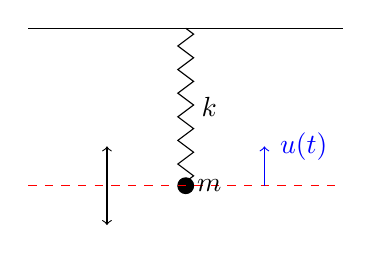
\begin{tikzpicture}
\draw[decoration = {zigzag,segment length = 3mm, amplitude = 1mm},decorate] (3,3) -- (3,1);
\filldraw[color=black] (3,1) circle (0.1);
\draw[color=red,dashed] (1,1) -- (5,1);
\path(3.3,2) [black] node {$k$};
\draw (1,3) -- (5,3);
\draw[->] (2,1) -- (2,1.5);
\draw[->] (2,1) -- (2,0.5);
\path(3.3,1) [black] node {$m$};
\draw[color=blue,->] (4,1) -- (4,1.5);
\path(4.5,1.5) [blue] node {$u(t)$};
\end{tikzpicture}
\caption{A body oscillating on a spring.}
\end{figure}
\end{center}
\item Equation of motion for harmonic oscillator
\vskip -30 pt
\begin{eqnarray*}
  \ddot{u}+\omega_{0}^{2}u&=&0 \\
  \omega_{0}^{2}&:=&\frac{k}{m}.
\end{eqnarray*}
\item This is one of the most important equation of motion in physics. It is present in every discipline, so we ought to solve it.

\pagebreak
\item One of our grandest method is to guess the solution. Let the solution be in the form $u(t)=e^{\lambda t}$, where $\lambda$ is an arbitrary parameter.
\begin{itemize}
\item $\dot{u}=\lambda e^{\lambda t}$, $\ddot{u}=\lambda^{2}e^{\lambda t}$
\item By substituting these assumption into equation, we gain
  $$ \left(\lambda^{2}+\omega_{0}^{2}\right)e^{\lambda t}=0.$$
\item Since the exponential function cannot be zero anywhere, we can divide by it, thus resulting an algeraic equation for $\lambda$
\begin{eqnarray*}
\lambda^{2}&=&-\omega_{0}^{2} \\
\lambda_{1,2}&=&\pm\omega_{0}i.
\end{eqnarray*}
\item We obtained not one, but two solutions
\vskip -10 pt
$$ u_{1}(t)=e^{i\omega_{0}t}, u_{2}(t)=e^{-i\omega_{0}t}.$$
\end{itemize}

\pagebreak
\item The general solution for equation of motion of umdamped harmonic oscillator is the sum of these two functions found above
\item General solution for harmonic oscillator's eq. of motion
$$u\left(t\right)=c_{1}e^{i\omega_{0}t}+c_{2}e^{-i\omega_{0}t},$$
where $c_{1},c_{2}$ are arbitrary parameters.
\item The general solution is \emph{complex} for a \emph{real} problem. Simple answer: No, it is not$\dots$. In order to see it, let us introduce \emph{initial conditions} for the situation. At $t=0$ the oscillating body has initial distance $u_{0}$ from the equilibrium position, furthermore initial velocity $v_{0}$, that is
\vskip -25 pt
  \begin{eqnarray*}
    u\left(0\right)&=&u_{0}\\
    \dot{u}\left(0\right)&=&v_{0}.
  \end{eqnarray*}
  \vskip -15 pt
These are initial conditions.

\pagebreak
\begin{eqnarray*}
I:u(0)&=&c_{1}+c_{2}=u_{0}, \\
II:\dot{u}(0)&=&i\omega_{0}\left(c_{1}-c_{2}\right)=v_{0}. \\
c_{1}&=&\frac{u_{0}}{2}+\frac{v_{0}}{2i\omega_{0}}, \\
c_{2}&=&\frac{u_{0}}{2}-\frac{v_{0}}{2i\omega_{0}}.
\end{eqnarray*}
$u(t)=c_{1}e^{i\omega_{0}t}+c_{2}e^{-i\omega_{0}t}=\left(\frac{u_{0}}{2}+\frac{v_{0}}{2i\omega_{0}}\right)e^{i\omega_{0}t}+\left(\frac{u_{0}}{2}-\frac{v_{0}}{2i\omega_{0}}\right)e^{-i\omega_{0}t}=u_{0}\left(\frac{e^{i\omega_{0}t}+e^{-i\omega_{0}t}}{2}\right)+\frac{v_{0}}{\omega_{0}}\left(\frac{e^{i\omega_{0}t}-e^{-i\omega_{0}t}}{2i}\right).$

\pagebreak
\item The particular solution for harmonic oscillator
$$\textcolor{blue}{u(t)=u_{0}\cos\omega_{0}t+\frac{v_{0}}{\omega_{0}}\sin\omega_{0}t}.$$
\item Here we have used connections between exponential and trigonometric functions: $\cos\phi=\frac{e^{i\phi}+e^{-i\phi}}{2}, \sin\phi=\frac{e^{i\phi}-e^{-i\phi}}{2i}$.
\end{itemize}

\end{frame}

% ----------------------------------------------------------------------------------------------------------------------------------------

\begin{frame}[fragile,squeeze,allowframebreaks]
\frametitle{Damped harmonic oscillator}
\begin{itemize}
\item Now we turn our attention to a more realistic situation, where there is friction in the system.
\begin{center}
\begin{figure}
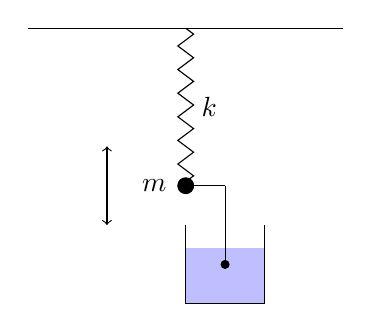
\begin{tikzpicture}
\draw[decoration = {zigzag,segment length = 3mm, amplitude = 1mm},decorate] (3,3) -- (3,1);
\filldraw[color=black] (3,1) circle (0.1);
\path(3.3,2) [black] node {$k$};
\draw (1,3) -- (5,3);
\draw[->] (2,1) -- (2,1.5);
\draw[->] (2,1) -- (2,0.5);
\path(2.6,1) [black] node {$m$};
\filldraw[color=blue!25] (3,-0.5) rectangle (4,0.2);
\draw (3.5,1) -- (3.5, 0);
\filldraw[color=black] (3.5,0) circle (0.05);
\draw (3,1) -- (3.5,1);
\draw (3,-0.5) -- (4,-0.5);
\draw (3,-0.5) -- (3,0.5);
\draw (4,-0.5) -- (4,0.5);
\end{tikzpicture}
\caption{Damped harmonic oscillator due to motion in water.}
\end{figure}
\end{center}
\item We consider the motion of harmonic oscillator damped due to a body moving in viscous fluid attached to the oscillator. The friction is proportional to the velocity.


\pagebreak
\item Equation of motion for damped oscillator
\begin{eqnarray*}
m\ddot{u}+c\dot{u}+ku&=&0, \\
\ddot{u}+2\beta\dot{u}+\omega_{0}^{2}u&=&0,
\end{eqnarray*}
where $2\beta=c/m, \omega_{0}^{2}=k/m$.
\item To obtain the solution, we use the previous method of guessing. We suppose that $u(t)=e^{i\omega t}$, where having learned from the previous case, we set $\lambda=i\omega$. Substituting the ansatz, we find
\begin{eqnarray*}
\left((i\omega)^{2}+2\beta i\omega+\omega_{0}^{2}\right)e^{i\omega t}&=&0, \\
\omega^{2}-2\beta i\omega-\omega_{0}^{2}&=&0,
\end{eqnarray*}

\pagebreak
where the two roots are
$$\omega_{1,2}=\frac{2\beta i\pm\sqrt{-4\beta^{2}+4\omega_{0}^{2}}}{2}=\beta i\pm\sqrt{\omega_{0}^{2}-\beta^{2}}=\beta i\pm\Omega.$$
\item General solution for eq. of motion is given by
\begin{eqnarray*}
u(t)&=&c_{1}e^{i\omega_{1}t}+c_{2}e^{i\omega_{2}t}, \\
u(t)&=&e^{-\beta t}\left(c_{1}e^{i\Omega t}+c_{2}e^{-i\Omega t}\right)
\end{eqnarray*}
\item By using the previous initial conditions $u(0)=u_{0}$, $\dot{u}(0)=v_{0}$, we receive the particular solution
  \vskip -20 pt
  $$u(t)=e^{-\beta t}\left(u_{0}\cos\omega_{0}t+\frac{v_{0}}{\omega_{0}}\sin\omega_{0}t\right).$$

\pagebreak
\item The solution decays exponentially. Of course, due to friction, the oscillation will stop eventually. In summary, we plot the two situations
\begin{center}
\begin{figure}
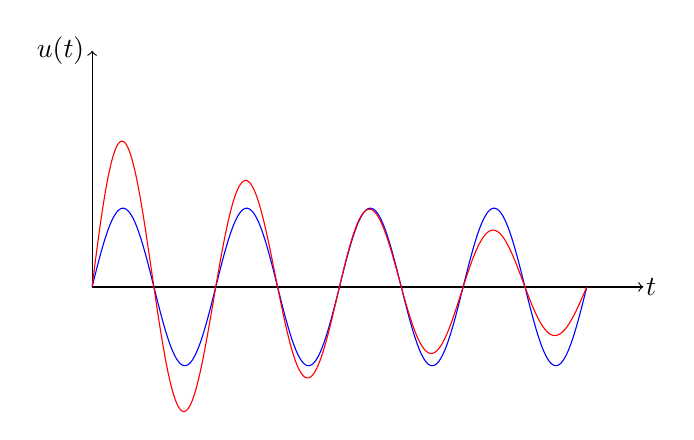
\begin{tikzpicture}[domain=0:4,samples=500,smooth]
\draw[->] (0,0) -- (7,0);
\draw[->] (0,0) -- (0,3);
\draw[color=blue, domain=0.001:2*pi]    plot (\x,{sin(4*\x r)});
\draw[color=red, domain=0.001:2*pi]    plot (\x,{2*exp(-0.2*\x)*sin(4*\x r)});
\path(7.1,0) [black] node {$t$};
\path(-0.4,3) [black] node {$u(t)$};
\end{tikzpicture}
\vskip -10 pt
\caption{An umdamped and a damped oscillator's evolution in time.}
\end{figure}
\end{center}

\pagebreak
\item Now, let us investigate the superposition of two harmonic oscillations. Oscillations are given by
\begin{eqnarray*}
  u_{1}(t)&=&A_{1}\sin\left(\omega t+\phi_{1}\right),\\
  u_{2}(t)&=&A_{2}\sin\left(\omega t+\phi_{2}\right).
\end{eqnarray*}
$A_{1},A_{2}$ are the \emph{amplitudes} and $\phi_{1},\phi_{2}$ are the \emph{initial phases}. What does the resulting oscillation look like?
\item We have used the trigonometric identity: $\sin(\alpha\pm\beta)=\sin\alpha\cos\beta\pm\cos\alpha\sin\beta$.
\item So, we got: $u(t)=A_{1}\sin\left(\omega t+\phi_{1}\right)+A_{2}\sin\left(\omega t+\phi_{2}\right)=A_{1}\left(\sin\omega t\cos\phi_{1}+\cos\omega t\sin\phi_{1}\right)+A_{2}\left(\sin\omega t\cos\phi_{2}+\cos\omega t\sin\phi_{2}\right)=\left(A_{1}\cos\phi_{1}+A_{2}\cos\phi_{2}\right)\sin\omega t+\left(A_{1}\sin\phi_{1}+A_{2}\sin\phi_{2}\right)\cos\omega t=A\cos\delta\sin\omega t+A\sin\delta\cos\omega t=A\sin\left(\omega t+\delta\right)$
\end{itemize}
\end{frame}

% ----------------------------------------------------------------------------------------------------------------------------------------

\begin{frame}
\frametitle{Harmonic oscillator: Superposition}
\begin{eqnarray*}
A\cos\delta&=&A_{1}\cos\phi_{1}+A_{2}\cos\phi_{2}, \\
A\sin\delta&=&A_{1}\sin\phi_{1}+A_{2}\sin\phi_{2},\\
A^{2}\cos^{2}\delta&=&A_{1}^{2}\cos^{2}\phi_{1}+2A_{1}A_{2}\cos\phi_{1}\cos\phi_{2}+A_{2}^{2}\cos^{2}\phi_{2} \\
A^{2}\sin^{2}\delta&=&A_{1}^{2}\sin^{2}\phi_{1}+2A_{1}A_{2}\sin\phi_{1}\sin\phi_{2}+A_{2}^{2}\sin^{2}\phi_{2} \\
A&=&\sqrt{A_{1}^{2}+A_{2}^{2}+2A_{1}A_{2}\cos(\phi_{1}-\phi_{2})}
\end{eqnarray*}             
\begin{itemize}
\item if $\phi_{1}=\phi_{2}$: $A=A_{1}+A_{2}$ \emph{constructive} oscillation
\item if $\vert\phi_{1}-\phi_{2}\vert=\pi$: $A=\vert A_{1}-A_{2}\vert$ \emph{destructive} oscillation
\end{itemize}
\end{frame}

% ----------------------------------------------------------------------------------------------------------------------------------------

\begin{frame}[fragile,squeeze,allowframebreaks]
\frametitle{Harmonic oscillator: Beat}
\begin{itemize}
\item As a last example for harmonic oscillations, we consider two oscillations with the same amplitude and phase, but with different frequencies
\item We have used the identity:$\sin\alpha+\sin\beta=2\cos\left(\frac{\alpha-\beta}{2}\right)\sin\left(\frac{\alpha+\beta}{2}\right)$
\begin{align*}
u_{1}(t)&=A\sin\omega_{1}, u_{2}(t)=A\sin\omega_{2}t.
\end{align*}
\begin{align*}
&u(t)=u_{1}(t)+u_{2}(t)=A\left(\sin\omega_{1}t+\sin\omega_{2}t\right)=\\
&=2A\cos\left(\frac{\omega_{1}-\omega_{2}}{2}t\right)\sin\left(\frac{\omega_{1}+\omega_{2}}{2}t\right).
\end{align*}
\item The resulting motion is a harmonic oscillation with oscillating amplitude: the phenomenon is called \emph{harmonic beat}.

\pagebreak
\begin{center}
\begin{figure}
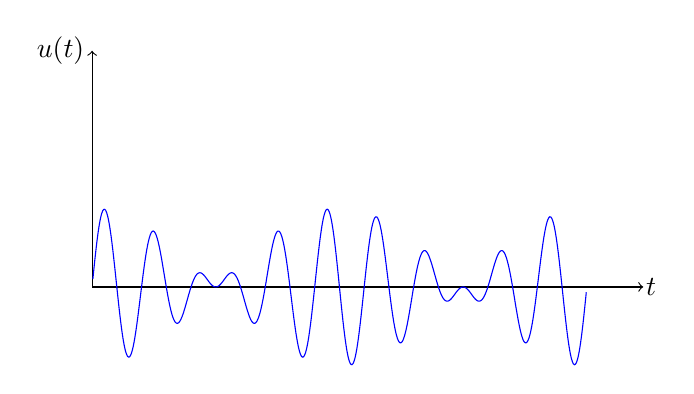
\begin{tikzpicture}[domain=0:4,samples=500,smooth]
\draw[->] (0,0) -- (7,0);
\draw[->] (0,0) -- (0,3);
\draw[color=blue,domain=0.01:2*pi]    plot (\x,{cos(\x r)*sin(10*\x r)});
\path(7.1,0) [black] node {$t$};
\path(-0.4,3) [black] node {$u(t)$};
\end{tikzpicture}
\caption{Harmonic beat}
\end{figure}
\end{center}

\end{itemize}
\end{frame}

% ----------------------------------------------------------------------------------------------------------------------------------------


% Definition Slide
\begin{frame}[fragile,squeeze,allowframebreaks]
  \frametitle{Resonance}
\begin{itemize}
\item Resonance is a phenomenon that occurs when a system is driven by an external periodic force at its \textbf{natural frequency} ($f_0$).
\begin{itemize}
\item When the driving frequency matches the natural frequency, the system oscillates with \textbf{maximum amplitude}.
\item At resonance, energy transfer from the external source to the system is most efficient.
\item It occurs in mechanical, acoustic, electrical, and atomic systems.
\end{itemize}

% Mathematical Background
\item The Driven Harmonic Oscillator: The motion of a damped, driven harmonic oscillator is described by:
\vskip -20 pt
\begin{equation*}
m\frac{d^2x}{dt^2} + b\frac{dx}{dt} + kx = F_0 \cos(\omega t)
\end{equation*}
\vskip -6 pt
\begin{itemize}
\item $m$: mass, $b$: damping coefficient, $k$: spring constant.
\item $F_0$: amplitude of the driving force.
\item $\omega$: angular frequency of the driving force.
\end{itemize}
\item Condition for Resonance: Resonance occurs when $\omega \approx \omega_0 = \sqrt{k/m}$.

\pagebreak  
% TikZ Diagram: Resonance Curve
\item The Resonance Curve
  \begin{center}
    \vskip -30 pt
    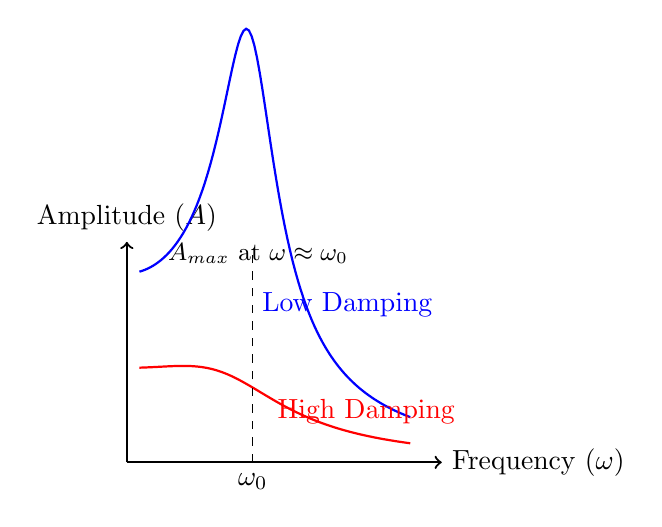
\begin{tikzpicture}[scale=0.8]
        % Axes
        \draw[->, thick] (0,0) -- (5,0) node[right] {Frequency ($\omega$)};
        \draw[->, thick] (0,0) -- (0,3.5) node[above] {Amplitude ($A$)};
        
        % Resonance curves (Low damping)
        \draw[blue, thick] plot [domain=0.2:4.5, samples=100] (\x, {3 / sqrt((1-\x^2/4)^2 + 0.05*\x^2)});
        \node[blue] at (3.5, 2.5) {Low Damping};
        
        % Resonance curves (High damping)
        \draw[red, thick] plot [domain=0.2:4.5, samples=100] (\x, {1.5 / sqrt((1-\x^2/4)^2 + 0.4*\x^2)});
        \node[red] at (3.8, 0.8) {High Damping};
        
        % Natural frequency marker
        \draw[dashed] (2,0) -- (2,3.3);
        \node at (2,-0.3) {$\omega_0$};
        
        % Labels
        \node[anchor=south west] at (0.5, 3) {\small $A_{max}$ at $\omega \approx \omega_0$};
    \end{tikzpicture}
    \end{center}
    \begin{itemize}
        \item \textbf{Peak}: Occurs at the natural frequency.
        \item \textbf{Damping}: Higher damping reduces the peak amplitude and widens the curve.
    \end{itemize}

\pagebreak
% Examples Slide
\item Real-World Examples
    \begin{columns}
        \column{0.5\textwidth}
        \textbf{Mechanical}
        \begin{itemize}
            \item Pushing a swing.
            \item Bridges collapsing (e.g., Tacoma Narrows).
        \end{itemize}
        
        \column{0.5\textwidth}
        \textbf{Acoustic/Electrical}
        \begin{itemize}
            \item Tuning a radio to a specific frequency.
            \item Musical instruments (body of a guitar).
        \end{itemize}
    \end{columns}
    \vspace{0.5cm}
\item Danger of Resonance: Uncontrolled resonance can lead to structural failure if the amplitude exceeds the material's elastic limit.

\end{itemize}
\end{frame}

% ----------------------------------------------------------------------------------------------------------------------------------------

\begin{frame}[fragile,squeeze,allowframebreaks]
\frametitle{Decomposition of periodic signals: Fourier theorem}
\begin{itemize}
\item We consider a signal in time $f(t)$, which has period $T$ meaning
$$f(t)=f(t+T).$$
\item How could we handle such a signal? We use functions, which we know well, trigonometric functions. The following functions have period $T$
\item We have defined frequency: $\omega_{1}=\frac{2\pi}{T}$.
\vskip -20 pt
\begin{eqnarray*}
      & & f(t)=1 \\
    f(t)=\sin\omega_{1}t&,&  f(t)=\cos\omega_{1}t \\
    f(t)=\sin2\omega_{1}t&,&  f(t)=\cos2\omega_{1}t \\
    \vdots && \vdots  \\
    f(t)=\sin n\omega_{1}t&,&  f(t)=\cos n\omega_{1}t \\
\end{eqnarray*}

\pagebreak
\begin{center}
\begin{figure}
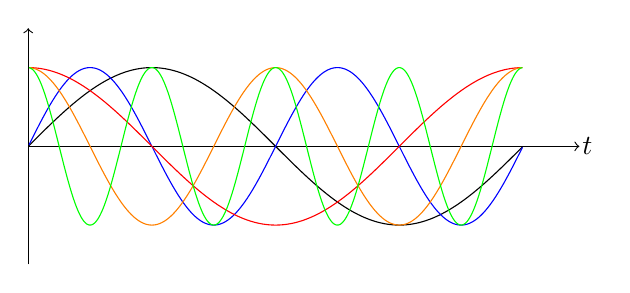
\begin{tikzpicture}[domain=0:4,samples=500,smooth]
\draw[->] (0,0) -- (7,0);
\draw[->] (0,-1.5) -- (0,1.5);
\draw[color=black,domain=0.01:2*pi]    plot (\x,{sin(\x r)});
\draw[color=blue,domain=0.01:2*pi]    plot (\x,{sin(2*\x r)});
\draw[color=red,domain=0.01:2*pi]    plot (\x,{cos(\x r)});
\draw[color=orange,domain=0.01:2*pi]    plot (\x,{cos(2*\x r)});
\draw[color=green,domain=0.01:2*pi]    plot (\x,{cos(4*\x r)});
\path(7.1,0) [black] node {$t$};
\end{tikzpicture}
\caption{Periodic harmonic signals with period $T$ and different frequencies.}
\end{figure}
\end{center}

\pagebreak
\item Fourier theorem: Any periodic signal can be decomposed as an infinite linear combination of trigonometric functions,
$$f(t)=a_{0}+\sum\limits_{k=1}^{\infty}a_{k}\cos k\omega_{1}t+\sum\limits_{k=1}^{\infty}b_{k}\sin k\omega_{1}t.$$
Where $a_{0},a_{k},b_{k}$ are called \emph{Fourier coefficients}.
\item It's quite annoying to memorize which coefficient relates to which trigonometric functions. So we do some magic with the help of complex functions. What does Euler's formula say?
\begin{eqnarray*}
e^{i\phi}&=&\cos\phi+i\sin\phi, \\
e^{-i\phi}&=&\cos\phi-i\sin\phi \\
\end{eqnarray*}

\pagebreak
$$\cos\phi=\frac{e^{i\phi}+e^{-i\phi}}{2}, \sin\phi=\frac{e^{i\phi}-e^{-i\phi}}{2i}.$$
\vskip -10 pt
\begin{itemize}
\item $a_{0}\rightarrow c_{0}$
\end{itemize}
$f(t)=c_{0}+\sum\limits_{k=1}^{\infty}a_{k}\cos k\omega_{1}t+\sum\limits_{k=1}^{\infty}b_{k}\sin k\omega_{1}t=c_{0}+\sum\limits_{k=1}^{\infty}a_{k}\left(\frac{e^{ik\omega_{1}t}+e^{-ik\omega_{1}t}}{2}\right)+\sum\limits_{k=1}^{\infty}b_{k}\left(\frac{e^{ik\omega_{1}t}-e^{-ik\omega_{1}t}}{2i}\right)=c_{0}e^{i0\omega_{1}t}+\sum\limits_{k=1}^{\infty}\left(\frac{a_{k}-ib_{k}}{2}\right)e^{ik\omega_{1}t}+\sum\limits_{k=1}^{\infty}\left(\frac{a_{k}+ib_{k}}{2}\right)e^{-ik\omega_{1}t}$
\begin{itemize}
\item $k>0:$ $c_{k}:=\frac{a_{k}-ib_{k}}{2}$, $k<0:$ $c_{k}:=\frac{a_{-k}+ib_{-k}}{2}$
\item in 2nd $\sum$: $k\rightarrow -k$
\end{itemize}
$$f(t)=c_{0}e^{i0\omega_{1}t}+\sum\limits_{k=1}^{\infty}c_{k}e^{ik\omega_{1}t}+\sum\limits_{k=-\infty}^{-1}c_{k}e^{ik\omega_{1}t},$$
\item Expressed in one, simple sum

\pagebreak
\item Fourier decomposition of periodic signal
  $$f(t)=\sum\limits_{k=-\infty}^{\infty}c_{k}e^{ik\omega_{1}t}.$$
\vskip -20 pt
\item How can we calculate the Fourier coefficients $c_{k}$? \\
$\int\limits_{-\frac{T}{2}}^{\frac{T}{2}}f(t)e^{-ik\omega_{1}t}dt=\int\limits_{-\frac{T}{2}}^{\frac{T}{2}}\sum\limits_{n=-\infty}^{\infty}c_{n}e^{in\omega_{1}t}e^{-ik\omega_{1}t}dt=\int\limits_{-\frac{T}{2}}^{\frac{T}{2}}\sum\limits_{n=-\infty}^{\infty}c_{n}e^{i(n-k)\omega_{1}t}dt=\sum\limits_{n=-\infty}^{\infty}c_{n}\int\limits_{-\frac{T}{2}}^{\frac{T}{2}}e^{i(n-k)\omega_{1}t}dt=\sum\limits_{n=-\infty}^{\infty}c_{n}\int\limits_{-\frac{T}{2}}^{\frac{T}{2}}\left(\cos(n-k)\omega_{1}t+i\sin(n-k)\omega_{1}t\right)dt=\sum\limits_{n=-\infty}^{\infty}c_{n}T\delta_{nk}=Tc_{k}$

\pagebreak
\item Therefore the Fourier coefficient
\begin{eqnarray*}
  c_{k}=\frac{1}{T}\int\limits_{-\frac{T}{2}}^{\frac{T}{2}}f(t)e^{-ik\omega_{1}t}&,&\delta_{nk}:=\begin{cases}
1, n=k \\
0, n\neq k \\
\end{cases},
\end{eqnarray*}
where $\delta_{nk}$ is called \emph{Kronecker delta symbol}.
\item Fourier theorem: Any periodic signal can be decomposed as linear combination of trigonometric functions
\begin{align*}
f(t)&=\sum\limits_{k=-\infty}^{\infty}c_{k}e^{ik\omega_{1}t},& c_{k}&=\frac{1}{T}\int\limits_{-\frac{T}{2}}^{\frac{T}{2}}f(t)e^{-ik\omega_{1}t}.
\end{align*}

\end{itemize}
\end{frame}

% ----------------------------------------------------------------------------------------------------------------------------------------

\begin{frame}[fragile,squeeze,allowframebreaks]
\frametitle{Decomposition of non-periodic signals: Fourier transform}
\begin{itemize}
\item What if we have to deal with non-periodic signals? Non-periodic signals can be obtained from periodic ones by taking $T\rightarrow\infty$.
\begin{eqnarray*}
  f(t)&=&\sum\limits_{k=-\infty}^{\infty}\left(\frac{c_{k}}{\Delta\omega}\right)e^{ik\omega_{1}t}\Delta\omega\\
  \frac{c_{k}}{\Delta\omega}&=&\frac{1}{2\pi}\int\limits_{-\frac{T}{2}}^{\frac{T}{2}}f(t)e^{-ik\omega_{1}t} \\
  \Delta\omega&=&(k+1)\omega_{1}-k\omega_{1}=\omega_{1}\\
  \lim\limits_{k\rightarrow\infty}k\omega_{1}=\omega &,& \Delta\omega \rightarrow d\omega
\end{eqnarray*}

\pagebreak
\item Fourier transform of non-periodic signals
\begin{eqnarray*}
  f(t)&=&\int\limits_{-\infty}^{\infty}F(\omega)e^{i\omega t}d\omega,\\
  F(\omega)&=&\frac{1}{2\pi}\int\limits_{-\infty}^{\infty}f(t)e^{-i\omega t}dt.
\end{eqnarray*}
\end{itemize}
\end{frame}


% ----------------------------------------------------------------------------------------------------------------------------------------

\begin{frame}
%\frametitle{Minden jó, ha a vége jó}

\vfill
\begin{center}
\textbf{\huge The End}

\bigskip
Thank you for your attention!
\end{center}
\vfill
\textbf{Acknowledgements} Thank you for the course materials for Szilárd~ZSÓKA and Zoltán~VARGA.
\end{frame}

\end{document}
